\documentclass[../thesis.tex]{subfiles}

\begin{document}

\chapter{Experiments}
\label{chap:exp}

\noindent In this chapter, we present the results of the experiments done in this thesis. The results are split into two sections. The first section presents the results from the cluster analysis and the second section that of the classification of clinical outcomes. For each of the sections we present an overview of the statistical learning problems that the algorithms are to solve. In this, we also present the assumptions and the evaluation criteria that are used to rank the algorithms and the final results. 

\section{Cluster analysis}

\noindent In the cluster analysis, we try to see how well the various clustering algorithms perform in producing phenotypically distinct clinical patient groups with HFpEF and HFmrEF. We organize this section in the following way: we start out by looking at the full sample data set, i.e. \texttt{HFfullDataSet.Rdat}. After the pre-processing, we will run the principal components thought the clustering algorithms. The idea is to see how well the clustering algorithms perform in producing patient groups that are more homogeneous compared to the physicians evaluation. Our measure of success is the number of unique baseline characteristics that are statistically significant using the Person $\chi^2$ test for categorical variables, ANOVA for normally distributed variables and Kruskal–Wallis test for non-normally distributed variables \citep{kruskal1952use}. All the tests are run using conventional levels of significance. The implementation is done using the \texttt{multigrps}-function from the \texttt{CBCgrps}-package in \texttt{r} \citep{CBCgrps}. The algorithms are performed on the binary clustering HF problem, i.e. to see how unique the patient groups produced are given that the only HF subtypes in the dataset is HFmrEF and HFpEF. This means that we assume a priori that there are only two clusters in the data set. After this we will see how well the algorithms perform in producing "new clusters" within the already defined patient groups from the first round. We will do the same analysis on both the groups that have been defined by the physicians and the "best" first round clustering algorithm. The full process flow for the cluster analysis is illustrated in Figure (\ref{fig:process_flow_clustering}).

\begin{figure}
    \centering
    \begin{minipage}[b]{\textwidth}

\centering
\normalsize
\tikzset{every picture/.style={line width=0.75pt}} %set default line width to 0.75pt        

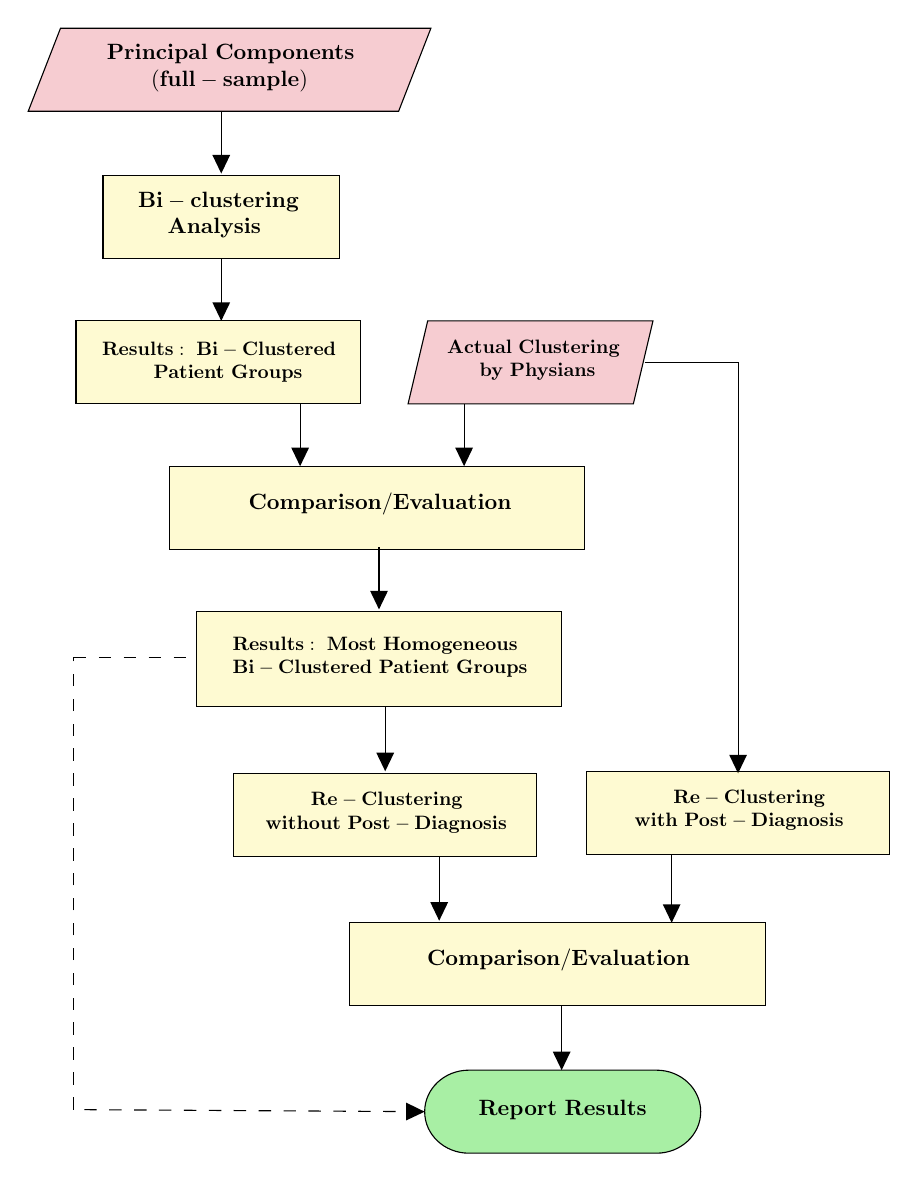
\begin{tikzpicture}[x=0.75pt,y=0.75pt,yscale=-1,xscale=1]
%uncomment if require: \path (0,606); %set diagram left start at 0, and has height of 606

%Shape: Parallelogram [id:dp6647145031150581] 
\draw  [fill={rgb, 255:red, 208; green, 2; blue, 27 }  ,fill opacity=0.2 ] (194.05,7) -- (372.5,7) -- (356.95,47) -- (178.5,47) -- cycle ;
%Straight Lines [id:da8846773602112543] 
\draw    (271.5,47) -- (271.5,75) ;
\draw [shift={(271.5,77)}, rotate = 270] [fill={rgb, 255:red, 0; green, 0; blue, 0 }  ][line width=0.75]  [draw opacity=0] (8.93,-4.29) -- (0,0) -- (8.93,4.29) -- cycle    ;

%Shape: Rectangle [id:dp27431555826277765] 
\draw  [fill={rgb, 255:red, 248; green, 231; blue, 28 }  ,fill opacity=0.2 ] (214.5,78) -- (328.5,78) -- (328.5,118) -- (214.5,118) -- cycle ;
%Straight Lines [id:da14961685906904876] 
\draw    (271.5,118) -- (271.5,146) ;
\draw [shift={(271.5,148)}, rotate = 270] [fill={rgb, 255:red, 0; green, 0; blue, 0 }  ][line width=0.75]  [draw opacity=0] (8.93,-4.29) -- (0,0) -- (8.93,4.29) -- cycle    ;

%Shape: Rectangle [id:dp09827610187608338] 
\draw  [fill={rgb, 255:red, 248; green, 231; blue, 28 }  ,fill opacity=0.2 ] (201.5,148) -- (338.5,148) -- (338.5,188) -- (201.5,188) -- cycle ;
%Straight Lines [id:da223473735957731] 
\draw    (309.5,188) -- (309.5,216) ;
\draw [shift={(309.5,218)}, rotate = 270] [fill={rgb, 255:red, 0; green, 0; blue, 0 }  ][line width=0.75]  [draw opacity=0] (8.93,-4.29) -- (0,0) -- (8.93,4.29) -- cycle    ;

%Straight Lines [id:da10156066919663931] 
\draw    (388.5,188) -- (388.5,216) ;
\draw [shift={(388.5,218)}, rotate = 270] [fill={rgb, 255:red, 0; green, 0; blue, 0 }  ][line width=0.75]  [draw opacity=0] (8.93,-4.29) -- (0,0) -- (8.93,4.29) -- cycle    ;

%Shape: Rectangle [id:dp1364397766049188] 
\draw  [fill={rgb, 255:red, 248; green, 231; blue, 28 }  ,fill opacity=0.2 ] (246.5,218) -- (446.5,218) -- (446.5,258) -- (246.5,258) -- cycle ;
%Straight Lines [id:da28849175814256767] 
\draw    (347.5,257) -- (347.5,285) ;
\draw [shift={(347.5,287)}, rotate = 270] [fill={rgb, 255:red, 0; green, 0; blue, 0 }  ][line width=0.75]  [draw opacity=0] (8.93,-4.29) -- (0,0) -- (8.93,4.29) -- cycle    ;

%Shape: Rectangle [id:dp855299838261038] 
\draw  [fill={rgb, 255:red, 248; green, 231; blue, 28 }  ,fill opacity=0.2 ] (259.5,288) -- (435.5,288) -- (435.5,334) -- (259.5,334) -- cycle ;
%Shape: Parallelogram [id:dp47004695097922267] 
\draw  [fill={rgb, 255:red, 208; green, 2; blue, 27 }  ,fill opacity=0.2 ] (370.96,148) -- (479.5,148) -- (470.04,188) -- (361.5,188) -- cycle ;
%Straight Lines [id:da06063407025060097] 
\draw    (475.5,168) -- (520.5,168) ;


%Straight Lines [id:da5926644195581223] 
\draw    (350.5,334) -- (350.5,363) ;
\draw [shift={(350.5,365)}, rotate = 270] [fill={rgb, 255:red, 0; green, 0; blue, 0 }  ][line width=0.75]  [draw opacity=0] (8.93,-4.29) -- (0,0) -- (8.93,4.29) -- cycle    ;

%Straight Lines [id:da8413098221287976] 
\draw    (520.5,168) -- (520.5,364) ;
\draw [shift={(520.5,366)}, rotate = 270] [fill={rgb, 255:red, 0; green, 0; blue, 0 }  ][line width=0.75]  [draw opacity=0] (8.93,-4.29) -- (0,0) -- (8.93,4.29) -- cycle    ;

%Shape: Rectangle [id:dp73563614757607] 
\draw  [fill={rgb, 255:red, 248; green, 231; blue, 28 }  ,fill opacity=0.2 ] (277.5,366) -- (423.5,366) -- (423.5,406) -- (277.5,406) -- cycle ;
%Shape: Rectangle [id:dp6744694293772151] 
\draw  [fill={rgb, 255:red, 248; green, 231; blue, 28 }  ,fill opacity=0.2 ] (333.5,438) -- (533.5,438) -- (533.5,478) -- (333.5,478) -- cycle ;
%Straight Lines [id:da43373610475282676] 
\draw    (376.5,406) -- (376.5,435) ;
\draw [shift={(376.5,437)}, rotate = 270] [fill={rgb, 255:red, 0; green, 0; blue, 0 }  ][line width=0.75]  [draw opacity=0] (8.93,-4.29) -- (0,0) -- (8.93,4.29) -- cycle    ;

%Straight Lines [id:da681049356627645] 
\draw    (488.5,405) -- (488.5,436) ;
\draw [shift={(488.5,438)}, rotate = 270] [fill={rgb, 255:red, 0; green, 0; blue, 0 }  ][line width=0.75]  [draw opacity=0] (8.93,-4.29) -- (0,0) -- (8.93,4.29) -- cycle    ;

%Straight Lines [id:da6627436883022095] 
\draw    (435.5,478) -- (435.5,507) ;
\draw [shift={(435.5,509)}, rotate = 270] [fill={rgb, 255:red, 0; green, 0; blue, 0 }  ][line width=0.75]  [draw opacity=0] (8.93,-4.29) -- (0,0) -- (8.93,4.29) -- cycle    ;

%Flowchart: Terminator [id:dp4539534632908053] 
\draw  [fill={rgb, 255:red, 139; green, 233; blue, 134 }  ,fill opacity=0.75 ] (390.78,509) -- (481.22,509) .. controls (492.97,509) and (502.5,517.95) .. (502.5,529) .. controls (502.5,540.05) and (492.97,549) .. (481.22,549) -- (390.78,549) .. controls (379.03,549) and (369.5,540.05) .. (369.5,529) .. controls (369.5,517.95) and (379.03,509) .. (390.78,509) -- cycle ;
%Straight Lines [id:da9928979089443342] 
\draw  [dash pattern={on 4.5pt off 4.5pt}]  (200.5,310) -- (259.5,310) ;


%Straight Lines [id:da9346137110249131] 
\draw  [dash pattern={on 4.5pt off 4.5pt}]  (200.5,528) -- (200.5,310) ;


%Straight Lines [id:da835721246834527] 
\draw  [dash pattern={on 4.5pt off 4.5pt}]  (367.5,528.99) -- (200.5,528) ;

\draw [shift={(369.5,529)}, rotate = 180.34] [fill={rgb, 255:red, 0; green, 0; blue, 0 }  ][line width=0.75]  [draw opacity=0] (8.93,-4.29) -- (0,0) -- (8.93,4.29) -- cycle    ;
%Shape: Rectangle [id:dp16102927554927304] 
\draw  [fill={rgb, 255:red, 248; green, 231; blue, 28 }  ,fill opacity=0.2 ] (447.5,365) -- (593.5,365) -- (593.5,405) -- (447.5,405) -- cycle ;

% Text Node
\draw (276,26) node [scale=0.8]  {$ \begin{array}{l}
\mathbf{Principal\ Components}\\
\ \ \ \ \ \ (\mathbf{full-sample})
\end{array}$};
% Text Node
\draw (272,97) node [scale=0.8]  {$ \begin{array}{l}
\mathbf{Bi-clustering\ }\\
\ \ \ \ \mathbf{Analysis}
\end{array}$};
% Text Node
\draw (272,168) node [scale=0.7]  {$ \begin{array}{l}
\mathbf{Results:\ Bi-Clustered\ }\\
\ \ \ \ \ \ \ \ \mathbf{Patient\ Groups}
\end{array}$};
% Text Node
\draw (422,167) node [scale=0.7]  {$ \begin{array}{l}
\mathbf{Actual\ Clustering}\\
\ \ \ \ \mathbf{\ by\ Physians}
\end{array}$};
% Text Node
\draw (348,236) node [scale=0.8]  {$\mathbf{Comparison/Evaluation}$};
% Text Node
\draw (348,310) node [scale=0.7]  {$ \begin{array}{l}
\mathbf{Results:\ Most\ Homogeneous}\\
\mathbf{Bi-Clustered\ Patient\ Groups}
\end{array}$};
% Text Node
\draw (351,385) node [scale=0.7]  {$ \begin{array}{l}
\ \ \ \ \ \ \ \mathbf{Re-Clustering\ }\\
\mathbf{without\ Post-Diagnosis}
\end{array}$};
% Text Node
\draw (434,456) node [scale=0.8]  {$\mathbf{Comparison/Evaluation}$};
% Text Node
\draw (436,528) node [scale=0.8]  {$\mathbf{Report\ Results}$};
% Text Node
\draw (521,384) node [scale=0.7]  {$ \begin{array}{l}
\ \ \ \ \ \ \mathbf{Re-Clustering\ }\\
\mathbf{with\ Post-Diagnosis}
\end{array}$};


\end{tikzpicture}

\end{minipage}
    \caption[Process flow clustering of patient groups]{\textit{Process flow clustering of patient groups}}
    \label{fig:process_flow_clustering}
\end{figure}

\subsection{The binary clustering HF problem}
\label{subsec:bi_clust}

The current clustering problem assumes that the dataset is only comprised of two clusters, i.e. HFmrEF and HFpEF. Accordingly, we allow the algorithms to determine the patients that best correspond to each cluster. We have plotted the results of the binary clustering problem in Figure (\ref{fig:bi_clust_results}). This plot can in many ways seem very misguiding as it only displays the results along the first two principal components. Still, the figure illustrates that even if we only cluster based on the first four principal components (27.32\% of variance explained), we can produce more distinct patient     

\begin{footnotesize}
\begin{tabularx}{1.2\textwidth}{LLLLp{1.7cm}p{3cm}}
\caption{Baseline characteristics of actual clustering}\label{tab:baseline_char_actual_full}\\
\toprule
& Total & Cluster1 & Cluster2 & $p$-value\\
\midrule
\endfirsthead
\caption*{\textbf{Table \ref{tab:baseline_char_actual_full}:} Baseline characteristics of actual clustering (\textit{continued})}\\
\toprule
& Total & Cluster1 & Cluster2 & $p$-value\\
\midrule
\endhead
hb & 109.34±20.29 & 107.85±21.22 & 110.93±19.18 & 0.141 \\ 
pcv & 0.34±0.06 & 0.33±0.06 & 0.34±0.06 & 0.159 \\ 
age & 78.64(69.22,84.17) & 78.9(69.46,85.37) & 78.08(68.73,82.74) & 0.141 \\ 
ewave & 0.9(0.74,1.05) & 0.92(0.8,1.1) & 0.9(0.7,1.01) & 0.056 \\ 
gfr & 48(32.5,70) & 47(32,72) & 51.96(33,67.77) & 0.968 \\ 
k & 4.4(4,4.7) & 4.4(4.1,4.7) & 4.4(4,4.78) & 0.664 \\ 
los & 10(4,22) & 10(4,22) & 10.5(4,21) & 0.880 \\ 
lvef & 50(45,57.5) & 57.5(55,60) & 45(42,47.5) & 0.000*** \\ 
mcv & 90.55(85.5,95) & 89(85,94) & 91.33(87,96) & 0.011** \\ 
na & 139(136,141) & 139(136,141) & 139(136,141) & 0.650 \\ 
ntprobnp & 2848(1230.5,7374) & 2217(997,5305) & 4063.5(1886.5,9968.25) & 0.000*** \\ 
plts & 204(156,268) & 217(163,284) & 190.87(148.5,241) & 0.003** \\ 
wbc & 7.8(5.9,10.5) & 7.6(6,10.5) & 8.1(5.9,10.4) & 0.727 \\ 
\midrule
\multicolumn{3}{l}{Total number of significant baseline char:} & 59\\
\multicolumn{3}{l}{\hspace*{0,5cm} Continuous: } & 4\\
\multicolumn{3}{l}{\hspace*{0,5cm} Categorical: } & 55\\
\midrule
\end{tabularx}
\end{footnotesize}

\begin{footnotesize}
\begin{tabularx}{1.2\textwidth}{LLLLp{1.7cm}p{3cm}}
\caption{Baseline characteristics of Hierarchical and K-Means clustering}\label{tab:baseline_char_actual_hckm}\\
\toprule
& Total & Cluster1 & Cluster2 & $p$-value\\
\midrule
\endfirsthead
\caption*{\textbf{Table \ref{tab:baseline_char_actual_hckm}:} Baseline characteristics of Hierarchical and K-Means clustering (\textit{continued})}\\
\toprule
& Total & Cluster1 & Cluster2 & $p$-value\\
\midrule
\endhead
hb & 109.34±20.29 & 106.79±21.29 & 111.73±19.06 & 0.019** \\ 
pcv & 0.34±0.06 & 0.33±0.07 & 0.35±0.06 & 0.035* \\ 
age & 78.64(69.22,84.17) & 78.9(68.94,85.36) & 78.26(69.73,82.8) & 0.416 \\ 
ewave & 0.9(0.74,1.05) & 0.97(0.8,1.1) & 0.9(0.7,1) & 0.002** \\ 
gfr & 48(32.5,70) & 46(31,70) & 54.44(34,71) & 0.205 \\ 
k & 4.4(4,4.7) & 4.4(4,4.7) & 4.4(4,4.8) & 0.219 \\ 
los & 10(4,22) & 10(4,22) & 11(4.25,21) & 0.889 \\ 
lvef & 50(45,57.5) & 57.5(52.5,60) & 45(42.5,47.5) & 0.000*** \\ 
mcv & 90.55(85.5,95) & 89(84,94) & 91.14(87,96) & 0.002** \\ 
na & 139(136,141) & 139(136,141) & 139(136,141) & 0.321 \\ 
ntprobnp & 2848(1230.5,7374) & 2327(1007,5695) & 3723.5(1731.5,9557.75) & 0.000*** \\ 
plts & 204(156,268) & 215(163,287) & 194(151,241) & 0.007** \\ 
wbc & 7.8(5.9,10.5) & 7.7(5.9,10.5) & 8.05(5.92,10.47) & 0.731 \\ 
\midrule
\multicolumn{3}{l}{Total number of significant baseline char:} & 62\\
\multicolumn{3}{l}{\hspace*{0,5cm} Continuous: } & 7\\
\multicolumn{3}{l}{\hspace*{0,5cm} Categorical: } & 55\\
\midrule
\end{tabularx}
\end{footnotesize}

\noindent groups than the physicians. As we can see from Table (\ref{tab:baseline_char_actual_hckm}), the hierarchical and k-means clustering algorithms both give the highest number of significant baseline characteristics (7 continuous and 55 categorical variables) compared with the actual clustering done by the physicians (4 continuous and 55 categorical variables, see Table \ref{tab:baseline_char_actual_full}). The EM algorithm produces overall the lowest number of significant baseline characteristics (5 continuous and 49 categorical variables). Both the hierarchical and k-means algorithm produce the same clustering configurations. The baseline characteristics in the clustering of the patients using the hierarchical and k-means clustering show that for the HFpEF cluster the \texttt{LVEF} is on average 57.5\% and for the second cluster (HFmrEF) the \texttt{LVEF} is on average 45\%. These are very similar values to what the physicians produced. We can also see that for other baseline characteristics such as \texttt{ntprobnp} the average is at 2327 ng/L for the HFpEF group which is significantly different than that of the HFmrEF group 3723.5 ng/L. This is also very similar to what the physicians concluded with. For characteristics that are significantly different in the clustering with hierarchical and k-means, but not found in the clustering done by the physicians one can include the following continuous variables: hemoglobin (\texttt{hb}), packed cell volume (\texttt{pcv}) and the ewave (\texttt{ewave}). This may suggest that both the hierarchical and k-means clustering algorithms    

\begin{footnotesize}
\begin{tabularx}{1.2\textwidth}{LLLLp{1.7cm}p{3cm}}
\caption{Baseline characteristics of EM clustering}\label{tab:baseline_char_actual_em}\\
\toprule
& Total & Cluster1 & Cluster2 & $p$-value\\
\midrule
\endfirsthead
\caption*{\textbf{Table \ref{tab:baseline_char_actual_em}:} Baseline characteristics of EM clustering (\textit{continued})}\\
\toprule
& Total & Cluster1 & Cluster2 & $p$-value\\
\midrule
\endhead
hb & 109.34±20.29 & 111.2±19.07 & 107.48±21.34 & 0.075 \\ 
pcv & 0.34±0.06 & 0.34±0.06 & 0.33±0.06 & 0.115 \\ 
age & 78.64(69.22,84.17) & 77.81(69.22,82.76) & 78.9(69.22,85.36) & 0.199 \\ 
ewave & 0.9(0.74,1.05) & 0.9(0.71,1.01) & 0.93(0.8,1.1) & 0.040* \\ 
gfr & 48(32.5,70) & 51.96(33,68.25) & 47(32,72) & 0.956 \\ 
k & 4.4(4,4.7) & 4.4(4,4.8) & 4.4(4,4.7) & 0.363 \\ 
los & 10(4,22) & 11(4,21) & 10(4,22) & 0.906 \\ 
lvef & 50(45,57.5) & 45(42,47.5) & 57.5(53.75,60) & 0.000*** \\ 
mcv & 90.55(85.5,95) & 91.14(87,96) & 89(84.5,94) & 0.007** \\ 
na & 139(136,141) & 139(136,141) & 139(136,141) & 0.330 \\ 
ntprobnp & 2848(1230.5,7374) & 3985(1849.5,10038.25) & 2226(990,5500) & 0.000*** \\ 
plts & 204(156,268) & 192.64(149.5,241.5) & 217(163.5,286) & 0.002** \\ 
wbc & 7.8(5.9,10.5) & 8.1(5.97,10.63) & 7.6(5.9,10.35) & 0.561 \\ 
\midrule
\multicolumn{3}{l}{Total number of significant baseline char:} & 54\\
\multicolumn{3}{l}{\hspace*{0,5cm} Continuous: } & 5\\
\multicolumn{3}{l}{\hspace*{0,5cm} Categorical: } & 49\\
\midrule
\end{tabularx}
\end{footnotesize}

\noindent can be used as appropriate tools for physicians. The results from the EM algorithm (Table \ref{tab:baseline_char_actual_em}) show that many of the similar baseline characteristics are not statistically significant. The LVEF (\texttt{lvef}) and NTproBNP (\texttt{ntprobnp}) are very similar to both the hierarchical and k-means clustering, but other characteristics such as hemoglobin (\texttt{hb}) and the packed cell volume (\texttt{pcv}) are not. Throughout the analysis we have found that the EM algorithm does not perform as well in clustering patient groups as the hierarchical and k-means clustering algorithms. This could be because the assumption of multivariate normal distribution does not hold for this data set or the fact that there is a high presence of categorical variables in the data set.

\subsection{Analysis of post-diagnosis}

\noindent In this section we will investigate the clustering results discussed previously. We have placed an assumption of whether the physicians diagnosis is representative given an objective of producing the most unique patient groups. The clustering problem in this section assumes that the diagnosis done by the physicians is sufficient in regards to this objective, i.e. the clustering based on the \textit{post-diagnosis} done by the physicians produces the  

\begin{footnotesize}
\begin{tabularx}{1.2\textwidth}{Lcccc}
\caption{Number of significant baseline characteristics}\label{tab:n_baseline}\\
\toprule
& \multicolumn{2}{c}{With Post-Diagnosis} & \multicolumn{2}{c}{Without Post-Diagnosis}\\
& HFpEF & HFmrEF & HFpEF & HFmrEF\\
\midrule
\endfirsthead
\caption*{\textbf{Table \ref{tab:n_baseline}:} Number of significant baseline characteristics (\textit{continued})}\\
\toprule
& \multicolumn{2}{c}{With Post-Diagnosis} & \multicolumn{2}{c}{Without Post-Diagnosis}\\
& HFpEF & HFmrEF & HFpEF & HFmrEF\\
\midrule
\endhead
Hierarchical &  53 (tab. \ref{tab:baseline_char_phy_p_hc}) &  53 (tab. \ref{tab:baseline_char_phy_mr_hc}) &  48 (tab. \ref{tab:baseline_char_nophy_p_hc}) &  51 (tab. \ref{tab:baseline_char_nophy_mr_hc})\\ 
K-Means &  49 (tab. \ref{tab:baseline_char_phy_p_km}) &  53 (tab. \ref{tab:baseline_char_phy_mr_km}) &  48 (tab. \ref{tab:baseline_char_nophy_p_km}) &  53 (tab. \ref{tab:baseline_char_nophy_mr_km})\\ 
EM &  56 (tab. \ref{tab:baseline_char_phy_p_em}) &  44 (tab. \ref{tab:baseline_char_phy_mr_em}) &  42 (tab. \ref{tab:baseline_char_nophy_p_em}) &  42 (tab. \ref{tab:baseline_char_nophy_mr_em})\\ 
\midrule
\end{tabularx}
\end{footnotesize}

\noindent most unique patient groups. We compare these results to a clustering without an assumption of post-diagnosis done by the physicians and see if there are any substantial differences in results. We will only use the first two principal components (14.64\% of variance explained) to cluster the patients. The evaluation criteria are the same as in the previous section. The number of clusters for the k-means and EM algorithm recommended by the \texttt{NbClust()} \citep{nbclust} function in \texttt{r} was three, i.e. 13 of the 23 indices in the procedure recommended using $C = 3$ as the optimal number of clusters for both the HFmrEF and HFpEF data sets. We can see from Table (\ref{tab:n_baseline}) that the hierarchical and k-means clustering algorithms produces the same number of significant baseline characteristics in half of the cases examined.  We can also see from Table (\ref{tab:n_baseline}) that all algorithms analyzed produce on average more statistically significant baseline characteristics with the post-diagnosis assumption compared to without. The EM algorithm produces overall the lowest number of significant baseline characteristics (in three cases). An exception is when the EM algorithm is clustering HFpEF with post-diagnosis.\\ 
\indent Beginning with the subtype HFpEF given the assumption of post-diagnosis, we can see from tables (\ref{tab:baseline_char_phy_p_hc}) and (\ref{tab:baseline_char_phy_p_km}) that cluster 2 (hierarchical \& k-means) seems to contain patients that have a higher average \texttt{age} (85.45) with a packed cell volume (\texttt{pcv}) that is on average 0.33 $\pm$ 0.05. This cluster is very similar to cluster 1 produced by the EM algorithm. The ntprobnp (\texttt{ntprobnp}) of cluster 3 (hierarchical \& k-means) is the lowest at 1417 ng/L which is also statistically significant. The average number of red blood cells, i.e. the mean corpusular volume (\texttt{mcv}) is at its lowest for cluster 1 (hierarchical \& k-means) with an average of 87 femtolitres. The number of significant baseline characteristics produced by the hierarchical clustering is 53 (8 cont. and 48 categorical) and for the k-means its 49 (8 cont. and 41 categorical). The EM algorithm produces almost similar results for the subgroup HFpEF as the hierarchical and k-means algorithm (table \ref{tab:baseline_char_phy_p_em}). The second cluster produced by the EM algorithm is very similar to the third cluster produced by the hierarchical and the k-means algorithm. The ntprobnp (\texttt{ntprobnp}) for cluster one and two produced by the EM are very similar. Both are approximately 2750 ng/L. The third cluster produced by the EM algorithm has the lowest values for the ntprobnp (1525 nl/L). The total number of significant baseline characteristics for the EM algorithm is 56 (8 cont. and 48 categorical). \\ 
\indent When looking at the HFmrEF clustering based on post-diagnosis (tables \ref{tab:baseline_char_phy_mr_hc}, \ref{tab:baseline_char_phy_mr_km} and \ref{tab:baseline_char_phy_mr_em}), we can see somewhat different results, i.e. there are on average less significantly different baseline characteristics in all clusters produced by the algorithms regardless of whether the assumption of post-diagnosis is intact. For cluster 3 (hierarchical and k-means), we find the lowest ntprobnp (\texttt{ntprobnp}) at 2898.5 ng/L with a packed cell volume of 0.38 $\pm$ 0.04. This cluster also contains the patients with the lowest length of stay (7 days). The length of stay (\texttt{LOS}) is also a uniquely statistically significant baseline characteristic that is only significant in the HFmrEF subgroup of patients for all algorithms studied. Cluster 3 also has the highest hemoglobin (\texttt{hb}) at 123.79 $\pm$ 12.89 g/100mL. The clustering results without the post-diagnosis assumption show very different results. In general, Figure (\ref{fig:clust_results_without_post_p}) and (\ref{fig:clust_results_without_post_mr}) show that the assignment of clustering have with very few similarities, i.e. the cluster numbering as well as the baseline characteristics vary more when the assumption of post-diagnosis is removed. Comparing the number of significant baseline characteristics between the HFmrEF groups both with and without the post-diagnosis assumption shows that the latter has on average fewer baseline characteristics, see Table (\ref{tab:n_baseline}). The same goes for the HFpEF group, i.e. we have reasons to believe that assuming the physicians diagnosis is representative, one can get additional clustered patient groups with higher degree of homogeneity compared to when this assumption is not intact. We have also demonstrated that the ML algorithms can be very useful in producing patient groups that are more phenotypically unique given that the objective is to challenge the diagnosis of the physicians, see section (\ref{subsec:bi_clust}). Now that we have presented the results of the clustering analysis, we move on to the results of the classification of the clinical outcomes. The source code, relevant plots and tables can be found in the appendix (\ref{chap:data_desc}).

\vspace*{-0,5cm}\section{Classification}

\noindent In this section we will present the results of the classification analysis. As mentioned in the ML procedure (Figure \ref{fig:ML_proc_thesis}), we train the algorithms using the imputed data sets and an iterative PCA and accordingly run cross validation in order to estimate the accuracy of the various algorithms. The accuracy along with Cohen’s kappa are the two evaluation criteria we use to rank the algorithms in this section. The process flow for the mentioned classification section is illustrated in Figure (\ref{fig:process_flow_classification}). 

\begin{figure}[!t]
    \centering
    \begin{minipage}[b]{\textwidth}

\centering
\normalsize

\tikzset{every picture/.style={line width=0.75pt}} %set default line width to 0.75pt        

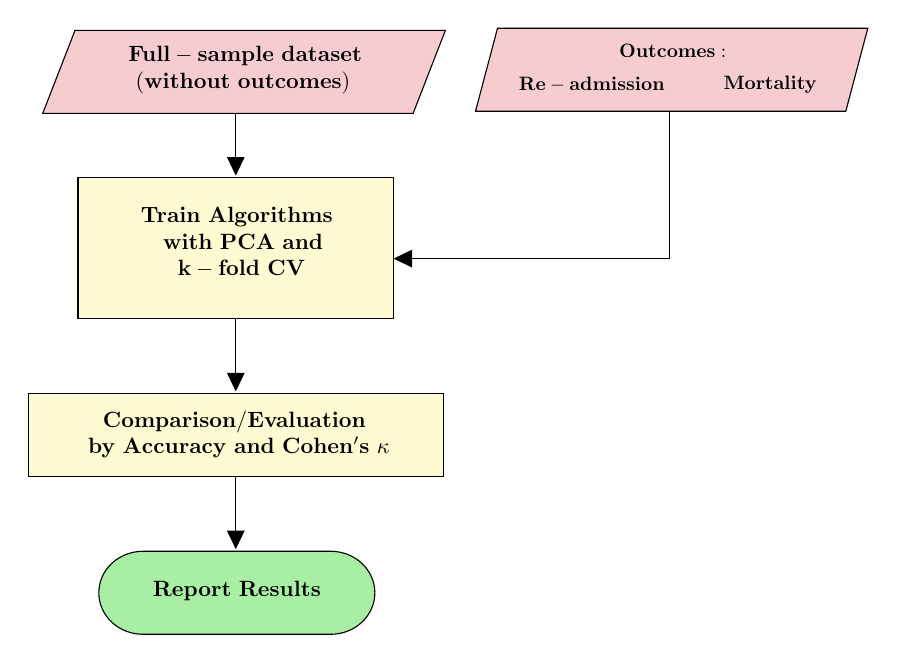
\begin{tikzpicture}[x=0.75pt,y=0.75pt,yscale=-1,xscale=1]
%uncomment if require: \path (0,401); %set diagram left start at 0, and has height of 401

%Shape: Parallelogram [id:dp1345085496641345] 
\draw  [fill={rgb, 255:red, 208; green, 2; blue, 27 }  ,fill opacity=0.2 ] (214.05,27) -- (392.5,27) -- (376.95,67) -- (198.5,67) -- cycle ;
%Straight Lines [id:da2529734460759472] 
\draw    (291.5,67) -- (291.5,95) ;
\draw [shift={(291.5,97)}, rotate = 270] [fill={rgb, 255:red, 0; green, 0; blue, 0 }  ][line width=0.75]  [draw opacity=0] (8.93,-4.29) -- (0,0) -- (8.93,4.29) -- cycle    ;

%Shape: Rectangle [id:dp8537246297754715] 
\draw  [fill={rgb, 255:red, 248; green, 231; blue, 28 }  ,fill opacity=0.2 ] (215.5,98) -- (367.5,98) -- (367.5,166) -- (215.5,166) -- cycle ;
%Shape: Parallelogram [id:dp3026993474655866] 
\draw  [fill={rgb, 255:red, 208; green, 2; blue, 27 }  ,fill opacity=0.2 ] (417.6,26) -- (596,26) -- (585.4,66) -- (407,66) -- cycle ;
%Straight Lines [id:da11621318058538299] 
\draw    (500.5,66) -- (500.5,137) ;


%Straight Lines [id:da5046262970656357] 
\draw    (369.5,137) -- (500.5,137) ;

\draw [shift={(367.5,137)}, rotate = 0] [fill={rgb, 255:red, 0; green, 0; blue, 0 }  ][line width=0.75]  [draw opacity=0] (8.93,-4.29) -- (0,0) -- (8.93,4.29) -- cycle    ;
%Shape: Rectangle [id:dp6205627904748299] 
\draw  [fill={rgb, 255:red, 248; green, 231; blue, 28 }  ,fill opacity=0.2 ] (191.5,202) -- (391.5,202) -- (391.5,242) -- (191.5,242) -- cycle ;
%Straight Lines [id:da7285903815225594] 
\draw    (291.5,166) -- (291.5,199) ;
\draw [shift={(291.5,201)}, rotate = 270] [fill={rgb, 255:red, 0; green, 0; blue, 0 }  ][line width=0.75]  [draw opacity=0] (8.93,-4.29) -- (0,0) -- (8.93,4.29) -- cycle    ;

%Straight Lines [id:da5366229358958934] 
\draw    (291.5,242) -- (291.5,275) ;
\draw [shift={(291.5,277)}, rotate = 270] [fill={rgb, 255:red, 0; green, 0; blue, 0 }  ][line width=0.75]  [draw opacity=0] (8.93,-4.29) -- (0,0) -- (8.93,4.29) -- cycle    ;

%Flowchart: Terminator [id:dp45661416532888843] 
\draw  [fill={rgb, 255:red, 139; green, 233; blue, 134 }  ,fill opacity=0.75 ] (246.78,278) -- (337.22,278) .. controls (348.97,278) and (358.5,286.95) .. (358.5,298) .. controls (358.5,309.05) and (348.97,318) .. (337.22,318) -- (246.78,318) .. controls (235.03,318) and (225.5,309.05) .. (225.5,298) .. controls (225.5,286.95) and (235.03,278) .. (246.78,278) -- cycle ;

% Text Node
\draw (296,46) node [scale=0.8]  {$ \begin{array}{l}
\mathbf{Full-sample\ dataset}\\
\mathbf{\ ( without\ outcomes)}
\end{array}$};
% Text Node
\draw (292,130) node [scale=0.8]  {$ \begin{array}{l}
\mathbf{Train\ Algorithms}\\
\ \ \ \mathbf{with\ PCA\ and\ }\\
\ \ \ \ \ \mathbf{k-fold\ CV}
\end{array}$};
% Text Node
\draw (463,53) node [scale=0.7]  {$\mathbf{Re-admission}$};
% Text Node
\draw (549,53) node [scale=0.7]  {$\mathbf{Mortality}$};
% Text Node
\draw (502,37) node [scale=0.7]  {$\mathbf{Outcomes:}$};
% Text Node
\draw (293,222) node [scale=0.8]  {$ \begin{array}{l}
\ \ \mathbf{Comparison/Evaluation}\\
\mathbf{by\ Accuracy\ and\ Cohen's\ \kappa }
\end{array}$};
% Text Node
\draw (292,297) node [scale=0.8]  {$\mathbf{Report\ Results}$};

\end{tikzpicture}


\end{minipage}
    \caption[Process flow classification of clinical outcomes]{\textit{Process flow classification of clinical outcomes}}
    \label{fig:process_flow_classification}
\end{figure}

\subsection{Mortality classifier}

\noindent The statistical learning problem in this section is a two-class classification problem where mortality is the clinical outcome in question. Our objective is to see how well the algorithms mentioned in Figure (\ref{fig:ML_proc_thesis}) perform in predicting the probability of mortality. We will train the algorithms using PCA and $10$-fold cross validation and evaluate the results using the accuracy, i.e. the proportion of true results and Cohen's kappa defined by:

\begin{align}
    \kappa \equiv \frac{p_0 - p_e}{1 - p_e}
\end{align}

\noindent where $p_0$ is the accuracy given by ${\mathit  {ACC}}=({\mathit  {TP}}+{\mathit  {TN}})/(P+N)$, and $p_e = 1 / N^2 \sum_{k} n_{k1}n_{k2}$, where $k$ is the number of categories / classes, $N$ the number of items and $n_{k1}$ the number of times rater $i$ predicted category $k$. $p_e$ is also referred to as the expected accuracy, i.e. what the accuracy that any \textit{random} classifier would be expected to achieve. Accordingly, Cohen's kappa is also regarded as the inter-rater agreement for qualitative (categorical) items, i.e. it is similar to the classification accuracy, except that it is normalized at the baseline of random chance on a dataset. A possible interpretation of this    

\begin{figure}[h!]
    \centering
    \scalebox{.8}{% Created by tikzDevice version 0.12 on 2018-11-08 15:03:43
% !TEX encoding = UTF-8 Unicode
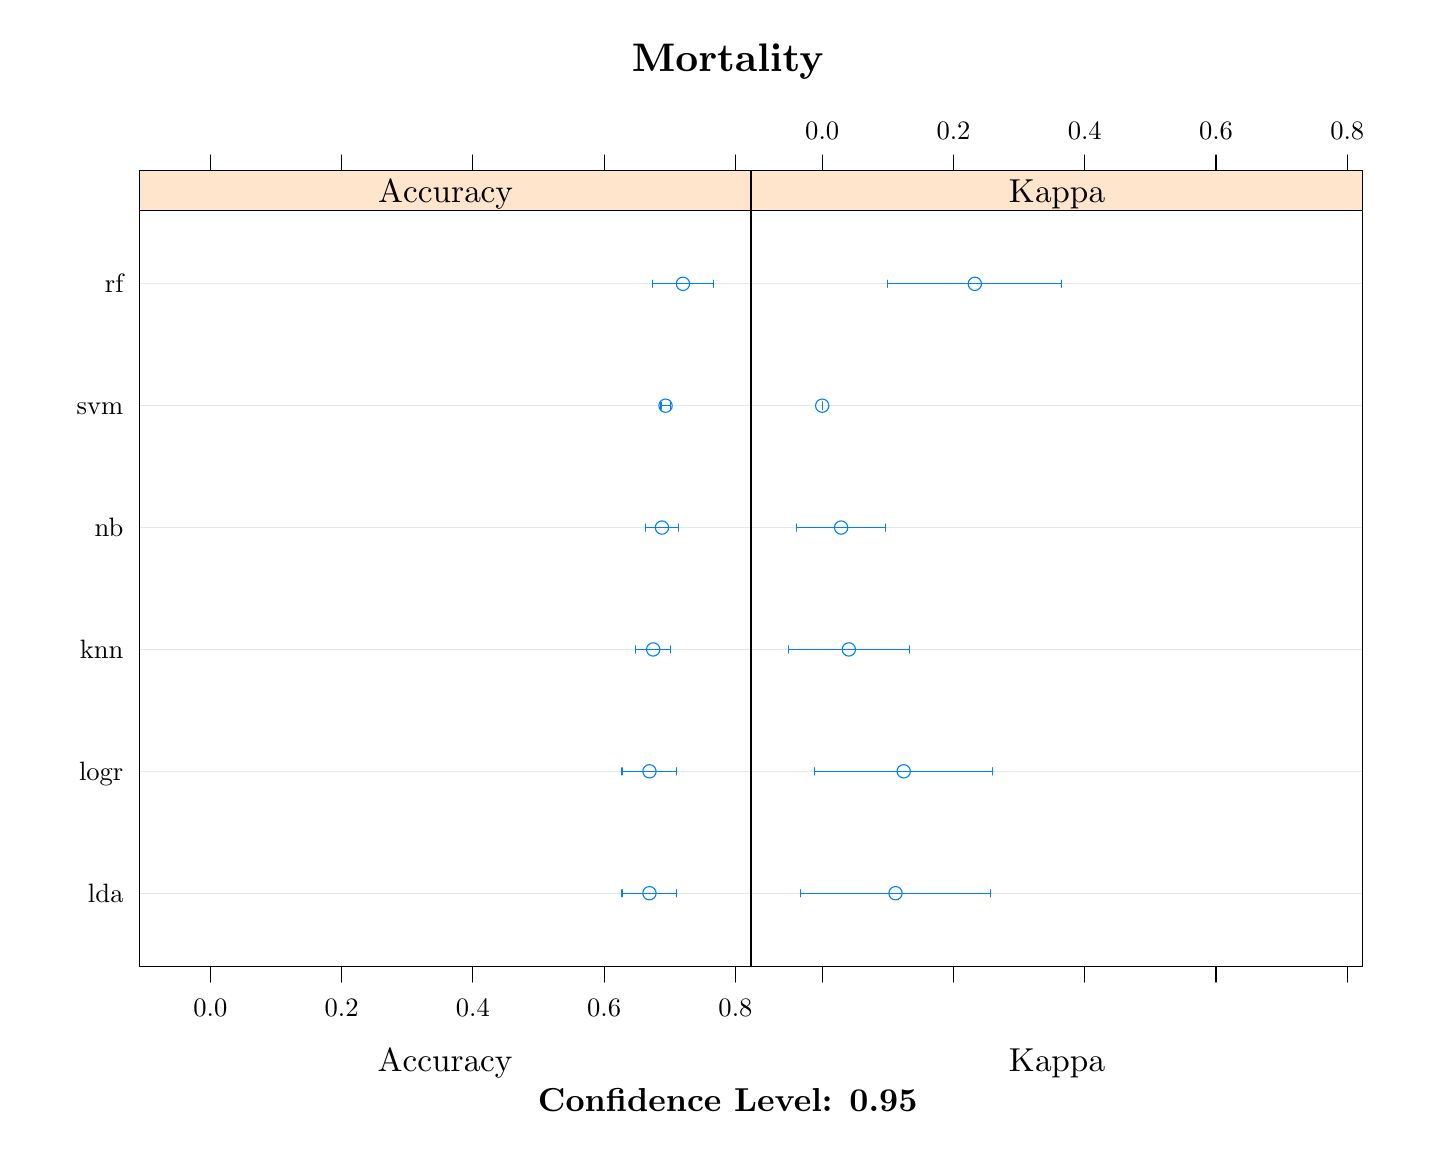
\begin{tikzpicture}[x=1pt,y=1pt]
\definecolor{fillColor}{RGB}{255,255,255}
\path[use as bounding box,fill=fillColor,fill opacity=0.00] (0,0) rectangle (505.89,397.48);
\begin{scope}
\path[clip] (  0.00,  0.00) rectangle (505.89,397.48);

\path[] (  0.00,  0.00) rectangle (505.89,397.48);
\definecolor{drawColor}{RGB}{0,0,0}

\node[text=drawColor,anchor=base,inner sep=0pt, outer sep=0pt, scale=  1.44] at (252.94,381.52) {\bfseries Mortality};
\end{scope}
\begin{scope}
\path[clip] (  0.00,  0.00) rectangle (505.89,397.48);
\definecolor{drawColor}{RGB}{0,0,0}

\node[text=drawColor,anchor=base,inner sep=0pt, outer sep=0pt, scale=  1.20] at (252.94,  6.02) {\bfseries Confidence Level: 0.95};
\end{scope}
\begin{scope}
\path[clip] (  0.00,  0.00) rectangle (505.89,397.48);
\definecolor{drawColor}{RGB}{0,0,0}

\node[text=drawColor,anchor=base,inner sep=0pt, outer sep=0pt, scale=  1.20] at (150.82, 20.33) {Accuracy};

\node[text=drawColor,anchor=base,inner sep=0pt, outer sep=0pt, scale=  1.20] at (371.92, 20.33) {Kappa};
\end{scope}
\begin{scope}
\path[clip] (  0.00,  0.00) rectangle (505.89,397.48);
\definecolor{drawColor}{RGB}{0,0,0}

\path[draw=drawColor,line width= 0.4pt,line join=round,line cap=round] ( 66.02,345.80) -- ( 66.02,351.49);

\path[draw=drawColor,line width= 0.4pt,line join=round,line cap=round] (113.45,345.80) -- (113.45,351.49);

\path[draw=drawColor,line width= 0.4pt,line join=round,line cap=round] (160.89,345.80) -- (160.89,351.49);

\path[draw=drawColor,line width= 0.4pt,line join=round,line cap=round] (208.32,345.80) -- (208.32,351.49);

\path[draw=drawColor,line width= 0.4pt,line join=round,line cap=round] (255.76,345.80) -- (255.76,351.49);
\end{scope}
\begin{scope}
\path[clip] (  0.00,  0.00) rectangle (505.89,397.48);
\definecolor{drawColor}{RGB}{0,0,0}

\node[text=drawColor,anchor=base east,inner sep=0pt, outer sep=0pt, scale=  0.96] at ( 34.58, 81.41) {lda};

\node[text=drawColor,anchor=base east,inner sep=0pt, outer sep=0pt, scale=  0.96] at ( 34.58,125.45) {logr};

\node[text=drawColor,anchor=base east,inner sep=0pt, outer sep=0pt, scale=  0.96] at ( 34.58,169.49) {knn};

\node[text=drawColor,anchor=base east,inner sep=0pt, outer sep=0pt, scale=  0.96] at ( 34.58,213.53) {nb};

\node[text=drawColor,anchor=base east,inner sep=0pt, outer sep=0pt, scale=  0.96] at ( 34.58,257.57) {svm};

\node[text=drawColor,anchor=base east,inner sep=0pt, outer sep=0pt, scale=  0.96] at ( 34.58,301.61) {rf};
\end{scope}
\begin{scope}
\path[clip] (  0.00,  0.00) rectangle (505.89,397.48);
\definecolor{drawColor}{RGB}{0,0,0}

\path[draw=drawColor,line width= 0.4pt,line join=round,line cap=round] ( 66.02, 58.30) -- ( 66.02, 52.61);

\path[draw=drawColor,line width= 0.4pt,line join=round,line cap=round] (113.45, 58.30) -- (113.45, 52.61);

\path[draw=drawColor,line width= 0.4pt,line join=round,line cap=round] (160.89, 58.30) -- (160.89, 52.61);

\path[draw=drawColor,line width= 0.4pt,line join=round,line cap=round] (208.32, 58.30) -- (208.32, 52.61);

\path[draw=drawColor,line width= 0.4pt,line join=round,line cap=round] (255.76, 58.30) -- (255.76, 52.61);

\node[text=drawColor,anchor=base,inner sep=0pt, outer sep=0pt, scale=  0.96] at ( 66.02, 40.30) {0.0};

\node[text=drawColor,anchor=base,inner sep=0pt, outer sep=0pt, scale=  0.96] at (113.45, 40.30) {0.2};

\node[text=drawColor,anchor=base,inner sep=0pt, outer sep=0pt, scale=  0.96] at (160.89, 40.30) {0.4};

\node[text=drawColor,anchor=base,inner sep=0pt, outer sep=0pt, scale=  0.96] at (208.32, 40.30) {0.6};

\node[text=drawColor,anchor=base,inner sep=0pt, outer sep=0pt, scale=  0.96] at (255.76, 40.30) {0.8};
\end{scope}
\begin{scope}
\path[clip] ( 40.28, 58.30) rectangle (261.37,331.34);
\definecolor{drawColor}{RGB}{230,230,230}

\path[draw=drawColor,line width= 0.4pt,line join=round,line cap=round] ( 40.28, 84.72) -- (261.37, 84.72);

\path[draw=drawColor,line width= 0.4pt,line join=round,line cap=round] ( 40.28,128.76) -- (261.37,128.76);

\path[draw=drawColor,line width= 0.4pt,line join=round,line cap=round] ( 40.28,172.80) -- (261.37,172.80);

\path[draw=drawColor,line width= 0.4pt,line join=round,line cap=round] ( 40.28,216.84) -- (261.37,216.84);

\path[draw=drawColor,line width= 0.4pt,line join=round,line cap=round] ( 40.28,260.88) -- (261.37,260.88);

\path[draw=drawColor,line width= 0.4pt,line join=round,line cap=round] ( 40.28,304.92) -- (261.37,304.92);
\definecolor{drawColor}{RGB}{0,128,255}

\path[draw=drawColor,line width= 0.4pt,line join=round,line cap=round] (224.68, 84.72) circle (  2.41);

\path[draw=drawColor,line width= 0.4pt,line join=round,line cap=round] (224.68,128.76) circle (  2.41);

\path[draw=drawColor,line width= 0.4pt,line join=round,line cap=round] (226.03,172.80) circle (  2.41);

\path[draw=drawColor,line width= 0.4pt,line join=round,line cap=round] (229.20,216.84) circle (  2.41);

\path[draw=drawColor,line width= 0.4pt,line join=round,line cap=round] (230.49,260.88) circle (  2.41);

\path[draw=drawColor,line width= 0.4pt,line join=round,line cap=round] (236.78,304.92) circle (  2.41);

\path[draw=drawColor,line width= 0.4pt,line join=round,line cap=round] (214.77, 84.72) -- (234.60, 84.72);

\path[draw=drawColor,line width= 0.4pt,line join=round,line cap=round] (214.77,128.76) -- (234.60,128.76);

\path[draw=drawColor,line width= 0.4pt,line join=round,line cap=round] (219.76,172.80) -- (232.31,172.80);

\path[draw=drawColor,line width= 0.4pt,line join=round,line cap=round] (223.27,216.84) -- (235.14,216.84);

\path[draw=drawColor,line width= 0.4pt,line join=round,line cap=round] (228.83,260.88) -- (232.14,260.88);

\path[draw=drawColor,line width= 0.4pt,line join=round,line cap=round] (225.76,304.92) -- (247.79,304.92);

\path[draw=drawColor,line width= 0.4pt,line join=round,line cap=round] (214.77, 86.04) -- (214.77, 83.40);

\path[draw=drawColor,line width= 0.4pt,line join=round,line cap=round] (214.77,130.08) -- (214.77,127.44);

\path[draw=drawColor,line width= 0.4pt,line join=round,line cap=round] (219.76,174.12) -- (219.76,171.48);

\path[draw=drawColor,line width= 0.4pt,line join=round,line cap=round] (223.27,218.16) -- (223.27,215.52);

\path[draw=drawColor,line width= 0.4pt,line join=round,line cap=round] (228.83,262.20) -- (228.83,259.56);

\path[draw=drawColor,line width= 0.4pt,line join=round,line cap=round] (225.76,306.24) -- (225.76,303.60);

\path[draw=drawColor,line width= 0.4pt,line join=round,line cap=round] (234.60, 86.04) -- (234.60, 83.40);

\path[draw=drawColor,line width= 0.4pt,line join=round,line cap=round] (234.60,130.08) -- (234.60,127.44);

\path[draw=drawColor,line width= 0.4pt,line join=round,line cap=round] (232.31,174.12) -- (232.31,171.48);

\path[draw=drawColor,line width= 0.4pt,line join=round,line cap=round] (235.14,218.16) -- (235.14,215.52);

\path[draw=drawColor,line width= 0.4pt,line join=round,line cap=round] (232.14,262.20) -- (232.14,259.56);

\path[draw=drawColor,line width= 0.4pt,line join=round,line cap=round] (247.79,306.24) -- (247.79,303.60);
\end{scope}
\begin{scope}
\path[clip] (  0.00,  0.00) rectangle (505.89,397.48);
\definecolor{drawColor}{RGB}{0,0,0}

\path[draw=drawColor,line width= 0.4pt,line join=round,line cap=round] ( 40.28, 58.30) rectangle (261.37,331.34);
\end{scope}
\begin{scope}
\path[clip] ( 40.28,331.34) rectangle (261.37,345.80);
\definecolor{drawColor}{RGB}{255,229,204}
\definecolor{fillColor}{RGB}{255,229,204}

\path[draw=drawColor,line width= 0.4pt,line join=round,line cap=round,fill=fillColor] ( 40.28,331.34) rectangle (261.37,345.80);
\definecolor{drawColor}{RGB}{0,0,0}

\node[text=drawColor,anchor=base west,inner sep=0pt, outer sep=0pt, scale=  1.20] at (126.65,334.44) {Accuracy};
\end{scope}
\begin{scope}
\path[clip] (  0.00,  0.00) rectangle (505.89,397.48);
\definecolor{drawColor}{RGB}{0,0,0}

\path[draw=drawColor,line width= 0.4pt,line join=round,line cap=round] ( 40.28,331.34) rectangle (261.37,345.80);
\end{scope}
\begin{scope}
\path[clip] (  0.00,  0.00) rectangle (505.89,397.48);
\definecolor{drawColor}{RGB}{0,0,0}

\path[draw=drawColor,line width= 0.4pt,line join=round,line cap=round] (287.11,345.80) -- (287.11,351.49);

\path[draw=drawColor,line width= 0.4pt,line join=round,line cap=round] (334.55,345.80) -- (334.55,351.49);

\path[draw=drawColor,line width= 0.4pt,line join=round,line cap=round] (381.98,345.80) -- (381.98,351.49);

\path[draw=drawColor,line width= 0.4pt,line join=round,line cap=round] (429.41,345.80) -- (429.41,351.49);

\path[draw=drawColor,line width= 0.4pt,line join=round,line cap=round] (476.85,345.80) -- (476.85,351.49);

\node[text=drawColor,anchor=base,inner sep=0pt, outer sep=0pt, scale=  0.96] at (287.11,357.18) {0.0};

\node[text=drawColor,anchor=base,inner sep=0pt, outer sep=0pt, scale=  0.96] at (334.55,357.18) {0.2};

\node[text=drawColor,anchor=base,inner sep=0pt, outer sep=0pt, scale=  0.96] at (381.98,357.18) {0.4};

\node[text=drawColor,anchor=base,inner sep=0pt, outer sep=0pt, scale=  0.96] at (429.41,357.18) {0.6};

\node[text=drawColor,anchor=base,inner sep=0pt, outer sep=0pt, scale=  0.96] at (476.85,357.18) {0.8};
\end{scope}
\begin{scope}
\path[clip] (  0.00,  0.00) rectangle (505.89,397.48);
\definecolor{drawColor}{RGB}{0,0,0}

\path[draw=drawColor,line width= 0.4pt,line join=round,line cap=round] (287.11, 58.30) -- (287.11, 52.61);

\path[draw=drawColor,line width= 0.4pt,line join=round,line cap=round] (334.55, 58.30) -- (334.55, 52.61);

\path[draw=drawColor,line width= 0.4pt,line join=round,line cap=round] (381.98, 58.30) -- (381.98, 52.61);

\path[draw=drawColor,line width= 0.4pt,line join=round,line cap=round] (429.41, 58.30) -- (429.41, 52.61);

\path[draw=drawColor,line width= 0.4pt,line join=round,line cap=round] (476.85, 58.30) -- (476.85, 52.61);
\end{scope}
\begin{scope}
\path[clip] (261.37, 58.30) rectangle (482.46,331.34);
\definecolor{drawColor}{RGB}{230,230,230}

\path[draw=drawColor,line width= 0.4pt,line join=round,line cap=round] (261.37, 84.72) -- (482.46, 84.72);

\path[draw=drawColor,line width= 0.4pt,line join=round,line cap=round] (261.37,128.76) -- (482.46,128.76);

\path[draw=drawColor,line width= 0.4pt,line join=round,line cap=round] (261.37,172.80) -- (482.46,172.80);

\path[draw=drawColor,line width= 0.4pt,line join=round,line cap=round] (261.37,216.84) -- (482.46,216.84);

\path[draw=drawColor,line width= 0.4pt,line join=round,line cap=round] (261.37,260.88) -- (482.46,260.88);

\path[draw=drawColor,line width= 0.4pt,line join=round,line cap=round] (261.37,304.92) -- (482.46,304.92);
\definecolor{drawColor}{RGB}{0,128,255}

\path[draw=drawColor,line width= 0.4pt,line join=round,line cap=round] (313.59, 84.72) circle (  2.41);

\path[draw=drawColor,line width= 0.4pt,line join=round,line cap=round] (316.55,128.76) circle (  2.41);

\path[draw=drawColor,line width= 0.4pt,line join=round,line cap=round] (296.72,172.80) circle (  2.41);

\path[draw=drawColor,line width= 0.4pt,line join=round,line cap=round] (293.93,216.84) circle (  2.41);

\path[draw=drawColor,line width= 0.4pt,line join=round,line cap=round] (287.11,260.88) circle (  2.41);

\path[draw=drawColor,line width= 0.4pt,line join=round,line cap=round] (342.25,304.92) circle (  2.41);

\path[draw=drawColor,line width= 0.4pt,line join=round,line cap=round] (279.27, 84.72) -- (347.90, 84.72);

\path[draw=drawColor,line width= 0.4pt,line join=round,line cap=round] (284.38,128.76) -- (348.72,128.76);

\path[draw=drawColor,line width= 0.4pt,line join=round,line cap=round] (274.95,172.80) -- (318.49,172.80);

\path[draw=drawColor,line width= 0.4pt,line join=round,line cap=round] (277.74,216.84) -- (310.12,216.84);

\path[draw=drawColor,line width= 0.4pt,line join=round,line cap=round] (287.11,260.88) -- (287.11,260.88);

\path[draw=drawColor,line width= 0.4pt,line join=round,line cap=round] (310.84,304.92) -- (373.65,304.92);

\path[draw=drawColor,line width= 0.4pt,line join=round,line cap=round] (279.27, 86.04) -- (279.27, 83.40);

\path[draw=drawColor,line width= 0.4pt,line join=round,line cap=round] (284.38,130.08) -- (284.38,127.44);

\path[draw=drawColor,line width= 0.4pt,line join=round,line cap=round] (274.95,174.12) -- (274.95,171.48);

\path[draw=drawColor,line width= 0.4pt,line join=round,line cap=round] (277.74,218.16) -- (277.74,215.52);

\path[draw=drawColor,line width= 0.4pt,line join=round,line cap=round] (287.11,262.20) -- (287.11,259.56);

\path[draw=drawColor,line width= 0.4pt,line join=round,line cap=round] (310.84,306.24) -- (310.84,303.60);

\path[draw=drawColor,line width= 0.4pt,line join=round,line cap=round] (347.90, 86.04) -- (347.90, 83.40);

\path[draw=drawColor,line width= 0.4pt,line join=round,line cap=round] (348.72,130.08) -- (348.72,127.44);

\path[draw=drawColor,line width= 0.4pt,line join=round,line cap=round] (318.49,174.12) -- (318.49,171.48);

\path[draw=drawColor,line width= 0.4pt,line join=round,line cap=round] (310.12,218.16) -- (310.12,215.52);

\path[draw=drawColor,line width= 0.4pt,line join=round,line cap=round] (287.11,262.20) -- (287.11,259.56);

\path[draw=drawColor,line width= 0.4pt,line join=round,line cap=round] (373.65,306.24) -- (373.65,303.60);
\end{scope}
\begin{scope}
\path[clip] (  0.00,  0.00) rectangle (505.89,397.48);
\definecolor{drawColor}{RGB}{0,0,0}

\path[draw=drawColor,line width= 0.4pt,line join=round,line cap=round] (261.37, 58.30) rectangle (482.46,331.34);
\end{scope}
\begin{scope}
\path[clip] (261.37,331.34) rectangle (482.46,345.80);
\definecolor{drawColor}{RGB}{255,229,204}
\definecolor{fillColor}{RGB}{255,229,204}

\path[draw=drawColor,line width= 0.4pt,line join=round,line cap=round,fill=fillColor] (261.37,331.34) rectangle (482.46,345.80);
\definecolor{drawColor}{RGB}{0,0,0}

\node[text=drawColor,anchor=base west,inner sep=0pt, outer sep=0pt, scale=  1.20] at (354.59,334.44) {Kappa};
\end{scope}
\begin{scope}
\path[clip] (  0.00,  0.00) rectangle (505.89,397.48);
\definecolor{drawColor}{RGB}{0,0,0}

\path[draw=drawColor,line width= 0.4pt,line join=round,line cap=round] (261.37,331.34) rectangle (482.46,345.80);
\end{scope}
\end{tikzpicture}
}
    \caption[Binary classification results: mortality]{\textit{Binary classification results: mortality}}
    \label{fig:bi_class_mort}
\end{figure}

\newpage
\noindent statistics is given by the following \citep{ashby1991practical}: less than 0.20 = Poor agreement, 0.20 to 0.40 = Fair agreement, 0.40 to 0.60 = Moderate agreement, 0.60 to 0.80 = Good agreement and 0.80 to 1 = Very good agreement. As mentioned earlier, the statistical learning problem is a binary classification problem given by whether  readmission / mortality occurred (\texttt{TRUE}) or not (\texttt{FALSE}), i.e. the expected accuracy is $p_e = 0.50$. We use principal component analysis to address the problem of higher dimensional multi-correlated variables. Accordingly, in the process of training the algorithms we use all principal components from the training in the classification of the clinical outcomes. The total number of patients with post-confirmed mortality in this data set is 115 (approx 36\% of the total number of patients, see Table \ref{tab:outcomes_class}). The results of the mortality classification is illustrated in Figure (\ref{fig:bi_class_mort}) and Table (\ref{tab:class_mortality}). In the table we notice that there are three algorithms that overall yield very decent results given the accuracy and the kappa. These are in order of importance: linear discriminant analysis (\texttt{lda}), logistic regression (\texttt{logr}) and naive Bayes (\texttt{nb}). As we can see the LDA (\texttt{lda}) produces the best overall accuracy and kappa. The mean accuracy of the LDA classifier is estimated at 69.9\% with a kappa at 0.19. The next classifier which compared to LDA also yields decent results is the logistic regression (\texttt{logr}) with a

\begin{footnotesize}
\begin{tabularx}{\textwidth}{LLLLLLLL}
\caption{Summary statistics for the mortality classification}\label{tab:class_mortality}\\
\toprule
 & Min. & 1st Qu. & Median & Mean & 3rd Qu. & Max. & NA's \\ 
\midrule
\endfirsthead
\caption*{\textbf{Table \ref{tab:class_mortality}:} Summary statistics mortality classification (\textit{continued})}\\
\toprule
 & Min. & 1st Qu. & Median & Mean & 3rd Qu. & Max. & NA's \\ 
\midrule
\endhead
\multicolumn{8}{c}{PANEL I: Accuracy}\\
\midrule
knn & 0.622 & 0.651 & 0.667 & 0.675 & 0.709 & 0.730 & 0.000 \\ 
logr & 0.568 & 0.628 & 0.680 & 0.669 & 0.709 & 0.763 & 0.000 \\ 
lda & 0.568 & 0.628 & 0.680 & 0.669 & 0.709 & 0.763 & 0.000 \\ 
nb & 0.649 & 0.658 & 0.684 & 0.688 & 0.723 & 0.737 & 0.000 \\ 
svm & 0.684 & 0.684 & 0.693 & 0.693 & 0.703 & 0.703 & 0.000 \\ 
rf & 0.595 & 0.703 & 0.711 & 0.720 & 0.745 & 0.838 & 0.000 \\
\midrule
\multicolumn{8}{c}{PANEL II: Kappa}\\
\midrule
knn & -0.146 & -0.027 & 0.013 & 0.041 & 0.100 & 0.245 & 0.000 \\ 
logr & -0.228 & 0.012 & 0.149 & 0.124 & 0.221 & 0.412 & 0.000 \\ 
lda & -0.228 & 0.000 & 0.121 & 0.112 & 0.257 & 0.412 & 0.000 \\ 
nb & -0.101 & -0.022 & 0.000 & 0.029 & 0.094 & 0.215 & 0.000 \\ 
svm & 0.000 & 0.000 & 0.000 & 0.000 & 0.000 & 0.000 & 0.000 \\ 
rf & -0.117 & 0.146 & 0.217 & 0.232 & 0.286 & 0.566 & 0.000 \\
\midrule
\end{tabularx}
\end{footnotesize}
\newpage
\noindent mean accuracy of 69.6\% and a kappa of 12. The last algorithm is the naive Bayes (\texttt{nb}). With the naive Bayes the estimated mean prediction accuracy of mortality is 66.4\% with a kappa of 0.098. We need to emphasize that even though one gets a somewhat high accuracy, the kappa is often considered to be a more robust evaluation criterion compared to the accuracy. This is because it takes into account that the agreement between estimated classification and actual classification can occur by chance. As the kappa is very low for all the classifiers mentioned in table (\ref{tab:class_mortality}), we cannot say with certainty that the classification algorithms can systematically predict mortality. However, we have reasons to believe that the three algorithms (linear discriminant analysis, logistic regression and naive Bayes) all show signs of being fair algorithms when it comes to predicting mortality in HF patients. Similar results are reported in the literature, see e.g. \cite{shah2014phenomapping} and \cite{panahiazar2015using}.

\subsection{Readmission classifier}

\noindent In this section, we examine the classification problem related to readmission. We have defined the readmission outcome as whether a given patient was re-admitted in some form during the one-year follow-up period. As we mentioned in section (\ref{sec:data}) this could be either within 30 days (patient group \texttt{V}) or any other way (patient groups \texttt{U}). The results of the readmission classification is illustrated in Figure (\ref{fig:bi_class_read}) and Table (\ref{tab:class_readmission}). The results are very different from what we found with the mortality classification. Surprisingly, three algorithms seem to distinguish themselves from the others, namely the linear discriminant analysis (\texttt{lda}), support vector machines (\texttt{svm}) and  

\vspace*{0,25cm}\begin{footnotesize}
\begin{tabularx}{\textwidth}{LLLLLLLL}
\caption{Summary statistics re-admission classification}\label{tab:class_readmission}\\
\toprule
 & Min. & 1st Qu. & Median & Mean & 3rd Qu. & Max. & NA's \\ 
\midrule
\endfirsthead
\caption*{\textbf{Table \ref{tab:class_readmission}:} Summary statistics re-admission classification (\textit{continued})}\\
\toprule
 & Min. & 1st Qu. & Median & Mean & 3rd Qu. & Max. & NA's \\ 
\midrule
\endhead
\multicolumn{8}{c}{PANEL I: Accuracy}\\
\midrule
knn & 0.595 & 0.609 & 0.654 & 0.658 & 0.698 & 0.737 & 0.000 \\ 
lda & 0.568 & 0.649 & 0.694 & 0.688 & 0.735 & 0.763 & 0.000 \\ 
nb & 0.838 & 0.921 & 0.960 & 0.947 & 0.974 & 1.000 & 0.000 \\ 
logr & 0.946 & 0.980 & 1.000 & 0.989 & 1.000 & 1.000 & 0.000 \\ 
svm & 0.973 & 1.000 & 1.000 & 0.997 & 1.000 & 1.000 & 0.000 \\ 
rf & 0.973 & 1.000 & 1.000 & 0.997 & 1.000 & 1.000 & 0.000 \\ 
\midrule
\multicolumn{8}{c}{PANEL II: Kappa}\\
\midrule
knn & -0.183 & -0.106 & 0.020 & 0.028 & 0.124 & 0.258 & 0.000 \\ 
lda & -0.101 & 0.037 & 0.193 & 0.168 & 0.327 & 0.408 & 0.000 \\ 
nb & 0.539 & 0.806 & 0.899 & 0.863 & 0.937 & 1.000 & 0.000 \\ 
logr & 0.877 & 0.955 & 1.000 & 0.975 & 1.000 & 1.000 & 0.000 \\ 
svm & 0.934 & 1.000 & 1.000 & 0.993 & 1.000 & 1.000 & 0.000 \\ 
rf & 0.934 & 1.000 & 1.000 & 0.993 & 1.000 & 1.000 & 0.000 \\
\midrule
\end{tabularx}
\end{footnotesize}

\noindent logistic regression (\texttt{logr}). Interestingly, all three of these algorithm score very high both in terms of accuracy and kappa. The algorithm with the most promising results is the linear discriminant analysis. It has an estimated mean prediction accuracy of 99.7\% with a kappa of 0.993. The LDA is found to be the most superior classification algorithm in both predicting mortality and readmission. The next algorithm that show potential in predicting readmission is the support vector machines (\texttt{svm}) algorithm. It has an estimated mean accuracy of 99.5\% with a kappa of 0.987. We consider this to be interesting as in the previous section we found that the SVM was one of the lowest performing algorithms when it comes to predicting mortality. This might suggest that modelling readmission with a non-linear structure is more realistic than doing so with mortality. The last algorithm that show potential is that of the logistic regression (\texttt{logr}). The estimated mean accuracy for this algorithm was 98.7\% with a kappa of 0.968. In addition to having a very good accuracy and kappa, its worth mentioning that given its level of simplicity, one can argue that the logistic regression algorithm is preferable to more advanced classification algorithms. This is not uncommon as in the literature there are many studies that report of logistic regression being a very effective algorithm for classifying clinical outcomes, see e.g. \cite{austin2013using} and \cite{zolfaghar2013big}. In both the cases that we have examined, we have found that the linear discriminant analysis and the logistic regression algorithms perform decently. These algorithms are very different in terms of their level of complexity. They are also very much used in the literature and often favourites among practitioners of medical statistical analysis, see e.g. \cite{austin2013using}, \cite{zolfaghar2013big}, \cite{shah2014phenomapping} and \cite{panahiazar2015using}. Accordingly, we have reasons to believe that the linear discriminant analysis and the logistic regression are the two algorithms that show the most potential in predicting both the mortality and readmission of HF patients.

\begin{figure}[th!]
    \centering
    \scalebox{.8}{% Created by tikzDevice version 0.12 on 2018-11-17 19:39:13
% !TEX encoding = UTF-8 Unicode
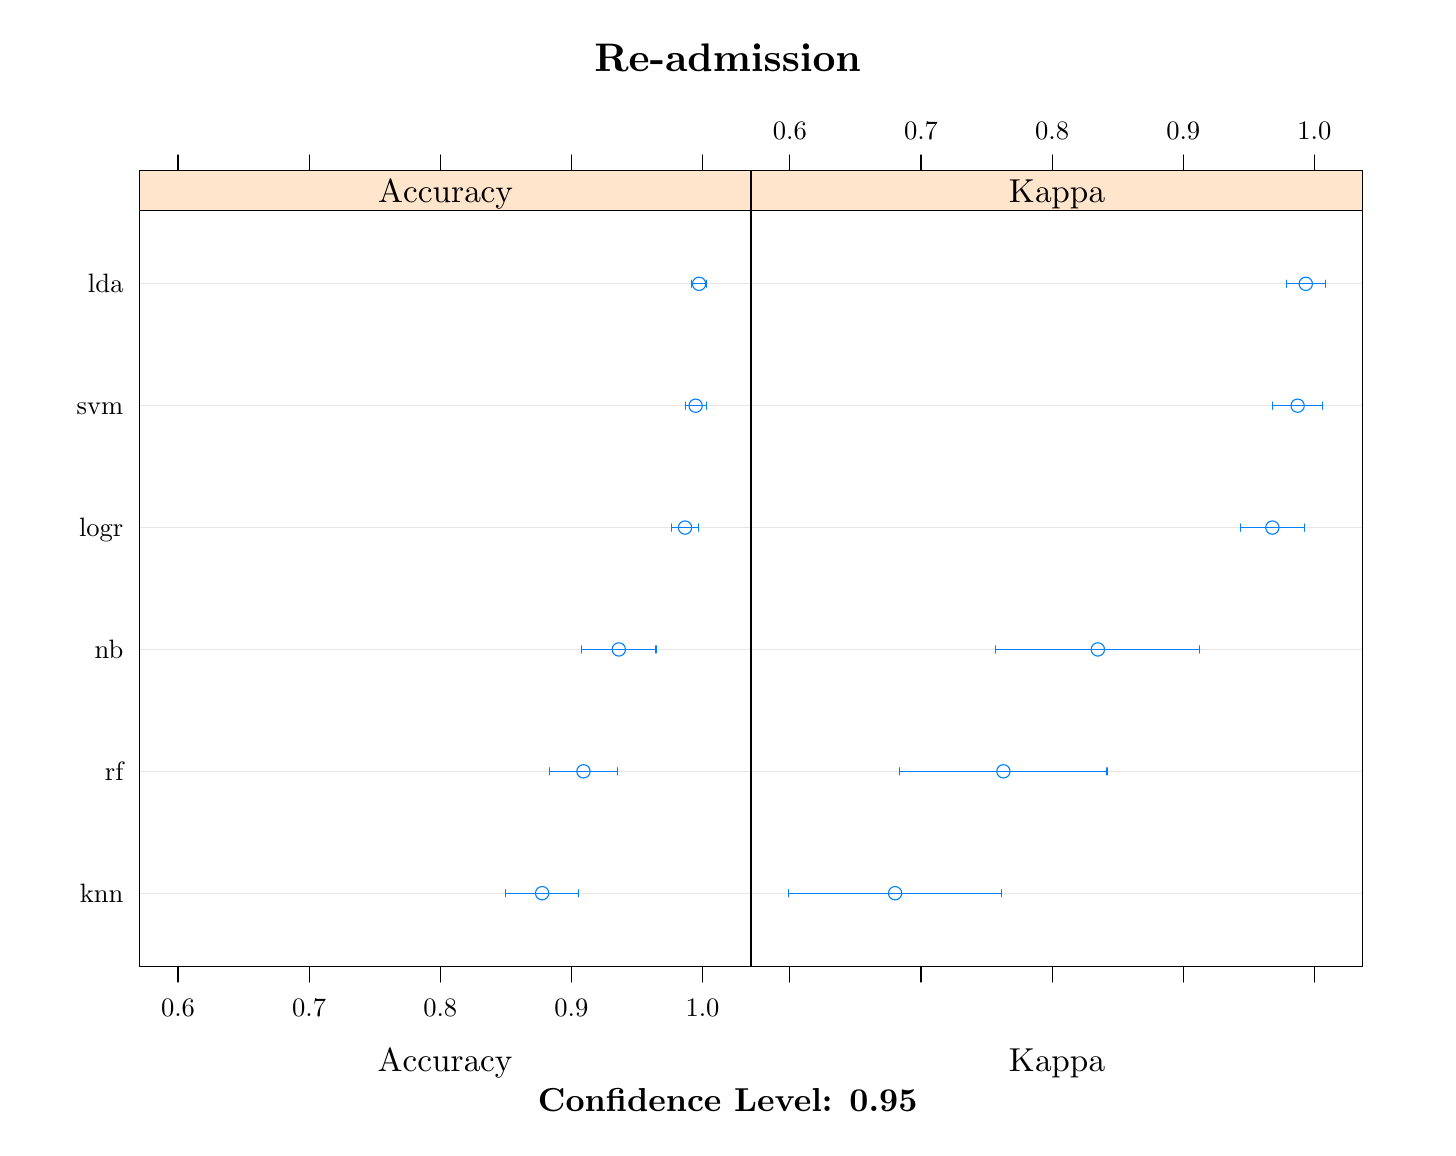
\begin{tikzpicture}[x=1pt,y=1pt]
\definecolor{fillColor}{RGB}{255,255,255}
\path[use as bounding box,fill=fillColor,fill opacity=0.00] (0,0) rectangle (505.89,397.48);
\begin{scope}
\path[clip] (  0.00,  0.00) rectangle (505.89,397.48);

\path[] (  0.00,  0.00) rectangle (505.89,397.48);
\definecolor{drawColor}{RGB}{0,0,0}

\node[text=drawColor,anchor=base,inner sep=0pt, outer sep=0pt, scale=  1.44] at (252.94,381.52) {\bfseries Re-admission};
\end{scope}
\begin{scope}
\path[clip] (  0.00,  0.00) rectangle (505.89,397.48);
\definecolor{drawColor}{RGB}{0,0,0}

\node[text=drawColor,anchor=base,inner sep=0pt, outer sep=0pt, scale=  1.20] at (252.94,  6.02) {\bfseries Confidence Level: 0.95};
\end{scope}
\begin{scope}
\path[clip] (  0.00,  0.00) rectangle (505.89,397.48);
\definecolor{drawColor}{RGB}{0,0,0}

\node[text=drawColor,anchor=base,inner sep=0pt, outer sep=0pt, scale=  1.20] at (150.82, 20.33) {Accuracy};

\node[text=drawColor,anchor=base,inner sep=0pt, outer sep=0pt, scale=  1.20] at (371.92, 20.33) {Kappa};
\end{scope}
\begin{scope}
\path[clip] (  0.00,  0.00) rectangle (505.89,397.48);
\definecolor{drawColor}{RGB}{0,0,0}

\path[draw=drawColor,line width= 0.4pt,line join=round,line cap=round] ( 54.33,345.80) -- ( 54.33,351.49);

\path[draw=drawColor,line width= 0.4pt,line join=round,line cap=round] (101.71,345.80) -- (101.71,351.49);

\path[draw=drawColor,line width= 0.4pt,line join=round,line cap=round] (149.10,345.80) -- (149.10,351.49);

\path[draw=drawColor,line width= 0.4pt,line join=round,line cap=round] (196.48,345.80) -- (196.48,351.49);

\path[draw=drawColor,line width= 0.4pt,line join=round,line cap=round] (243.86,345.80) -- (243.86,351.49);
\end{scope}
\begin{scope}
\path[clip] (  0.00,  0.00) rectangle (505.89,397.48);
\definecolor{drawColor}{RGB}{0,0,0}

\node[text=drawColor,anchor=base east,inner sep=0pt, outer sep=0pt, scale=  0.96] at ( 34.58, 81.41) {knn};

\node[text=drawColor,anchor=base east,inner sep=0pt, outer sep=0pt, scale=  0.96] at ( 34.58,125.45) {rf};

\node[text=drawColor,anchor=base east,inner sep=0pt, outer sep=0pt, scale=  0.96] at ( 34.58,169.49) {nb};

\node[text=drawColor,anchor=base east,inner sep=0pt, outer sep=0pt, scale=  0.96] at ( 34.58,213.53) {logr};

\node[text=drawColor,anchor=base east,inner sep=0pt, outer sep=0pt, scale=  0.96] at ( 34.58,257.57) {svm};

\node[text=drawColor,anchor=base east,inner sep=0pt, outer sep=0pt, scale=  0.96] at ( 34.58,301.61) {lda};
\end{scope}
\begin{scope}
\path[clip] (  0.00,  0.00) rectangle (505.89,397.48);
\definecolor{drawColor}{RGB}{0,0,0}

\path[draw=drawColor,line width= 0.4pt,line join=round,line cap=round] ( 54.33, 58.30) -- ( 54.33, 52.61);

\path[draw=drawColor,line width= 0.4pt,line join=round,line cap=round] (101.71, 58.30) -- (101.71, 52.61);

\path[draw=drawColor,line width= 0.4pt,line join=round,line cap=round] (149.10, 58.30) -- (149.10, 52.61);

\path[draw=drawColor,line width= 0.4pt,line join=round,line cap=round] (196.48, 58.30) -- (196.48, 52.61);

\path[draw=drawColor,line width= 0.4pt,line join=round,line cap=round] (243.86, 58.30) -- (243.86, 52.61);

\node[text=drawColor,anchor=base,inner sep=0pt, outer sep=0pt, scale=  0.96] at ( 54.33, 40.30) {0.6};

\node[text=drawColor,anchor=base,inner sep=0pt, outer sep=0pt, scale=  0.96] at (101.71, 40.30) {0.7};

\node[text=drawColor,anchor=base,inner sep=0pt, outer sep=0pt, scale=  0.96] at (149.10, 40.30) {0.8};

\node[text=drawColor,anchor=base,inner sep=0pt, outer sep=0pt, scale=  0.96] at (196.48, 40.30) {0.9};

\node[text=drawColor,anchor=base,inner sep=0pt, outer sep=0pt, scale=  0.96] at (243.86, 40.30) {1.0};
\end{scope}
\begin{scope}
\path[clip] ( 40.28, 58.30) rectangle (261.37,331.34);
\definecolor{drawColor}{RGB}{230,230,230}

\path[draw=drawColor,line width= 0.4pt,line join=round,line cap=round] ( 40.28, 84.72) -- (261.37, 84.72);

\path[draw=drawColor,line width= 0.4pt,line join=round,line cap=round] ( 40.28,128.76) -- (261.37,128.76);

\path[draw=drawColor,line width= 0.4pt,line join=round,line cap=round] ( 40.28,172.80) -- (261.37,172.80);

\path[draw=drawColor,line width= 0.4pt,line join=round,line cap=round] ( 40.28,216.84) -- (261.37,216.84);

\path[draw=drawColor,line width= 0.4pt,line join=round,line cap=round] ( 40.28,260.88) -- (261.37,260.88);

\path[draw=drawColor,line width= 0.4pt,line join=round,line cap=round] ( 40.28,304.92) -- (261.37,304.92);
\definecolor{drawColor}{RGB}{0,128,255}

\path[draw=drawColor,line width= 0.4pt,line join=round,line cap=round] (185.90, 84.72) circle (  2.41);

\path[draw=drawColor,line width= 0.4pt,line join=round,line cap=round] (200.83,128.76) circle (  2.41);

\path[draw=drawColor,line width= 0.4pt,line join=round,line cap=round] (213.60,172.80) circle (  2.41);

\path[draw=drawColor,line width= 0.4pt,line join=round,line cap=round] (237.53,216.84) circle (  2.41);

\path[draw=drawColor,line width= 0.4pt,line join=round,line cap=round] (241.37,260.88) circle (  2.41);

\path[draw=drawColor,line width= 0.4pt,line join=round,line cap=round] (242.61,304.92) circle (  2.41);

\path[draw=drawColor,line width= 0.4pt,line join=round,line cap=round] (172.76, 84.72) -- (199.03, 84.72);

\path[draw=drawColor,line width= 0.4pt,line join=round,line cap=round] (188.57,128.76) -- (213.08,128.76);

\path[draw=drawColor,line width= 0.4pt,line join=round,line cap=round] (200.17,172.80) -- (227.03,172.80);

\path[draw=drawColor,line width= 0.4pt,line join=round,line cap=round] (232.75,216.84) -- (242.30,216.84);

\path[draw=drawColor,line width= 0.4pt,line join=round,line cap=round] (237.61,260.88) -- (245.13,260.88);

\path[draw=drawColor,line width= 0.4pt,line join=round,line cap=round] (239.79,304.92) -- (245.44,304.92);

\path[draw=drawColor,line width= 0.4pt,line join=round,line cap=round] (172.76, 86.04) -- (172.76, 83.40);

\path[draw=drawColor,line width= 0.4pt,line join=round,line cap=round] (188.57,130.08) -- (188.57,127.44);

\path[draw=drawColor,line width= 0.4pt,line join=round,line cap=round] (200.17,174.12) -- (200.17,171.48);

\path[draw=drawColor,line width= 0.4pt,line join=round,line cap=round] (232.75,218.16) -- (232.75,215.52);

\path[draw=drawColor,line width= 0.4pt,line join=round,line cap=round] (237.61,262.20) -- (237.61,259.56);

\path[draw=drawColor,line width= 0.4pt,line join=round,line cap=round] (239.79,306.24) -- (239.79,303.60);

\path[draw=drawColor,line width= 0.4pt,line join=round,line cap=round] (199.03, 86.04) -- (199.03, 83.40);

\path[draw=drawColor,line width= 0.4pt,line join=round,line cap=round] (213.08,130.08) -- (213.08,127.44);

\path[draw=drawColor,line width= 0.4pt,line join=round,line cap=round] (227.03,174.12) -- (227.03,171.48);

\path[draw=drawColor,line width= 0.4pt,line join=round,line cap=round] (242.30,218.16) -- (242.30,215.52);

\path[draw=drawColor,line width= 0.4pt,line join=round,line cap=round] (245.13,262.20) -- (245.13,259.56);

\path[draw=drawColor,line width= 0.4pt,line join=round,line cap=round] (245.44,306.24) -- (245.44,303.60);
\end{scope}
\begin{scope}
\path[clip] (  0.00,  0.00) rectangle (505.89,397.48);
\definecolor{drawColor}{RGB}{0,0,0}

\path[draw=drawColor,line width= 0.4pt,line join=round,line cap=round] ( 40.28, 58.30) rectangle (261.37,331.34);
\end{scope}
\begin{scope}
\path[clip] ( 40.28,331.34) rectangle (261.37,345.80);
\definecolor{drawColor}{RGB}{255,229,204}
\definecolor{fillColor}{RGB}{255,229,204}

\path[draw=drawColor,line width= 0.4pt,line join=round,line cap=round,fill=fillColor] ( 40.28,331.34) rectangle (261.37,345.80);
\definecolor{drawColor}{RGB}{0,0,0}

\node[text=drawColor,anchor=base west,inner sep=0pt, outer sep=0pt, scale=  1.20] at (126.65,334.44) {Accuracy};
\end{scope}
\begin{scope}
\path[clip] (  0.00,  0.00) rectangle (505.89,397.48);
\definecolor{drawColor}{RGB}{0,0,0}

\path[draw=drawColor,line width= 0.4pt,line join=round,line cap=round] ( 40.28,331.34) rectangle (261.37,345.80);
\end{scope}
\begin{scope}
\path[clip] (  0.00,  0.00) rectangle (505.89,397.48);
\definecolor{drawColor}{RGB}{0,0,0}

\path[draw=drawColor,line width= 0.4pt,line join=round,line cap=round] (275.42,345.80) -- (275.42,351.49);

\path[draw=drawColor,line width= 0.4pt,line join=round,line cap=round] (322.81,345.80) -- (322.81,351.49);

\path[draw=drawColor,line width= 0.4pt,line join=round,line cap=round] (370.19,345.80) -- (370.19,351.49);

\path[draw=drawColor,line width= 0.4pt,line join=round,line cap=round] (417.57,345.80) -- (417.57,351.49);

\path[draw=drawColor,line width= 0.4pt,line join=round,line cap=round] (464.96,345.80) -- (464.96,351.49);

\node[text=drawColor,anchor=base,inner sep=0pt, outer sep=0pt, scale=  0.96] at (275.42,357.18) {0.6};

\node[text=drawColor,anchor=base,inner sep=0pt, outer sep=0pt, scale=  0.96] at (322.81,357.18) {0.7};

\node[text=drawColor,anchor=base,inner sep=0pt, outer sep=0pt, scale=  0.96] at (370.19,357.18) {0.8};

\node[text=drawColor,anchor=base,inner sep=0pt, outer sep=0pt, scale=  0.96] at (417.57,357.18) {0.9};

\node[text=drawColor,anchor=base,inner sep=0pt, outer sep=0pt, scale=  0.96] at (464.96,357.18) {1.0};
\end{scope}
\begin{scope}
\path[clip] (  0.00,  0.00) rectangle (505.89,397.48);
\definecolor{drawColor}{RGB}{0,0,0}

\path[draw=drawColor,line width= 0.4pt,line join=round,line cap=round] (275.42, 58.30) -- (275.42, 52.61);

\path[draw=drawColor,line width= 0.4pt,line join=round,line cap=round] (322.81, 58.30) -- (322.81, 52.61);

\path[draw=drawColor,line width= 0.4pt,line join=round,line cap=round] (370.19, 58.30) -- (370.19, 52.61);

\path[draw=drawColor,line width= 0.4pt,line join=round,line cap=round] (417.57, 58.30) -- (417.57, 52.61);

\path[draw=drawColor,line width= 0.4pt,line join=round,line cap=round] (464.96, 58.30) -- (464.96, 52.61);
\end{scope}
\begin{scope}
\path[clip] (261.37, 58.30) rectangle (482.46,331.34);
\definecolor{drawColor}{RGB}{230,230,230}

\path[draw=drawColor,line width= 0.4pt,line join=round,line cap=round] (261.37, 84.72) -- (482.46, 84.72);

\path[draw=drawColor,line width= 0.4pt,line join=round,line cap=round] (261.37,128.76) -- (482.46,128.76);

\path[draw=drawColor,line width= 0.4pt,line join=round,line cap=round] (261.37,172.80) -- (482.46,172.80);

\path[draw=drawColor,line width= 0.4pt,line join=round,line cap=round] (261.37,216.84) -- (482.46,216.84);

\path[draw=drawColor,line width= 0.4pt,line join=round,line cap=round] (261.37,260.88) -- (482.46,260.88);

\path[draw=drawColor,line width= 0.4pt,line join=round,line cap=round] (261.37,304.92) -- (482.46,304.92);
\definecolor{drawColor}{RGB}{0,128,255}

\path[draw=drawColor,line width= 0.4pt,line join=round,line cap=round] (313.44, 84.72) circle (  2.41);

\path[draw=drawColor,line width= 0.4pt,line join=round,line cap=round] (352.58,128.76) circle (  2.41);

\path[draw=drawColor,line width= 0.4pt,line join=round,line cap=round] (386.71,172.80) circle (  2.41);

\path[draw=drawColor,line width= 0.4pt,line join=round,line cap=round] (449.77,216.84) circle (  2.41);

\path[draw=drawColor,line width= 0.4pt,line join=round,line cap=round] (458.89,260.88) circle (  2.41);

\path[draw=drawColor,line width= 0.4pt,line join=round,line cap=round] (461.84,304.92) circle (  2.41);

\path[draw=drawColor,line width= 0.4pt,line join=round,line cap=round] (274.95, 84.72) -- (351.93, 84.72);

\path[draw=drawColor,line width= 0.4pt,line join=round,line cap=round] (315.14,128.76) -- (390.02,128.76);

\path[draw=drawColor,line width= 0.4pt,line join=round,line cap=round] (349.86,172.80) -- (423.57,172.80);

\path[draw=drawColor,line width= 0.4pt,line join=round,line cap=round] (438.31,216.84) -- (461.23,216.84);

\path[draw=drawColor,line width= 0.4pt,line join=round,line cap=round] (449.74,260.88) -- (468.04,260.88);

\path[draw=drawColor,line width= 0.4pt,line join=round,line cap=round] (454.79,304.92) -- (468.89,304.92);

\path[draw=drawColor,line width= 0.4pt,line join=round,line cap=round] (274.95, 86.04) -- (274.95, 83.40);

\path[draw=drawColor,line width= 0.4pt,line join=round,line cap=round] (315.14,130.08) -- (315.14,127.44);

\path[draw=drawColor,line width= 0.4pt,line join=round,line cap=round] (349.86,174.12) -- (349.86,171.48);

\path[draw=drawColor,line width= 0.4pt,line join=round,line cap=round] (438.31,218.16) -- (438.31,215.52);

\path[draw=drawColor,line width= 0.4pt,line join=round,line cap=round] (449.74,262.20) -- (449.74,259.56);

\path[draw=drawColor,line width= 0.4pt,line join=round,line cap=round] (454.79,306.24) -- (454.79,303.60);

\path[draw=drawColor,line width= 0.4pt,line join=round,line cap=round] (351.93, 86.04) -- (351.93, 83.40);

\path[draw=drawColor,line width= 0.4pt,line join=round,line cap=round] (390.02,130.08) -- (390.02,127.44);

\path[draw=drawColor,line width= 0.4pt,line join=round,line cap=round] (423.57,174.12) -- (423.57,171.48);

\path[draw=drawColor,line width= 0.4pt,line join=round,line cap=round] (461.23,218.16) -- (461.23,215.52);

\path[draw=drawColor,line width= 0.4pt,line join=round,line cap=round] (468.04,262.20) -- (468.04,259.56);

\path[draw=drawColor,line width= 0.4pt,line join=round,line cap=round] (468.89,306.24) -- (468.89,303.60);
\end{scope}
\begin{scope}
\path[clip] (  0.00,  0.00) rectangle (505.89,397.48);
\definecolor{drawColor}{RGB}{0,0,0}

\path[draw=drawColor,line width= 0.4pt,line join=round,line cap=round] (261.37, 58.30) rectangle (482.46,331.34);
\end{scope}
\begin{scope}
\path[clip] (261.37,331.34) rectangle (482.46,345.80);
\definecolor{drawColor}{RGB}{255,229,204}
\definecolor{fillColor}{RGB}{255,229,204}

\path[draw=drawColor,line width= 0.4pt,line join=round,line cap=round,fill=fillColor] (261.37,331.34) rectangle (482.46,345.80);
\definecolor{drawColor}{RGB}{0,0,0}

\node[text=drawColor,anchor=base west,inner sep=0pt, outer sep=0pt, scale=  1.20] at (354.59,334.44) {Kappa};
\end{scope}
\begin{scope}
\path[clip] (  0.00,  0.00) rectangle (505.89,397.48);
\definecolor{drawColor}{RGB}{0,0,0}

\path[draw=drawColor,line width= 0.4pt,line join=round,line cap=round] (261.37,331.34) rectangle (482.46,345.80);
\end{scope}
\end{tikzpicture}
}
    \caption[Binary classification results: readmission]{\textit{Binary classification results: readmission}}
    \label{fig:bi_class_read}
\end{figure}

\section{Discussion}

\noindent The objective of this thesis was two fold: (i) we attempted to give a though analysis of how well various clustering algorithms (hierarchical, k-means and expectation-maximization) perform in producing phenotypically distinct clinical patient groups (i.e. phenomapping) with HFpEF and HFmrEF. Our strategy for answering this research question has been to compare the level of dissimilarity between patient groups that are produced at two levels. Firstly, we looked at the binary clustering problem where we compared the patient groups produced by the algorithms with those produced by the physicians. We found that if one defines the optimal clustering as that which has the highest number of significantly different baseline characteristics, then we have reasons to believe that the hierarchical and k-means clustering algorithms show signs of being better at clustering patients with HF compared to the physicians. Overall these algorithms produce 62 significantly different baseline characteristics compared to 59 produced by the physicians. Secondly, we looked at how well the clustering algorithms performed in producing "new" patient groups within both subtypes of HF. We analyzed this by attempting to re-cluster patient groups from both subtypes (HFmrEF and HFpEF) produced by the physicians and the "best" ML algorithms. Re-clustering within the subtypes generated by the physicians (also called the 'post-diagnosis' assumption) seem to show the greatest potential as the average number of significantly different baseline characteristics is the highest for this clustering compared to when the assumption is removed. On average all algorithms produce approximately 53 (HFpEF) and 50 (HFmrEF) significantly different baseline characteristics when the post-diagnosis assumption is present compared to when its removed (46, HFpEF and 49, HFmrEF). However, if the objective is to use the results to find additional "new clusters", we cannot say with certainty that the choice of clustering algorithms or the clustering data used (whether it is with or without post-diagnosis) will systematically enhance the "uniqueness" of the patient groups. We need to emphasize that the results need to be treated with great caution as they are very sensitive to the number of principal components used, the imputation method and the sample size. Nevertheless, the hierarchical and k-means algorithms seems to have the potential to be used as tools by physicians to cross-check their assumptions and rational in order to further improve the diagnosis of patients with the preserved and mid-range subtypes of HF. Similar findings are also reported in the literature, see e.g. \cite{shah2014phenomapping}, \cite{ahmad2014clinical}, \cite{alonso2015exploring}, \cite{kao2015characterization}, \cite{ahmad2016clinical} and \cite{katz2017phenomapping}.\\
\indent In the second (ii) part of the thesis we attempted to evaluate the performance of various classification algorithms (k-nearest neighbour, logistic regression, linear discriminant analysis, support vector machines and random forest) in predicting mortality and readmission. The results suggest that linear discriminant analysis and logistic regression are good candidates for doing that. They both rank very high compared to the other algorithms evaluated. The LDA algorithm has an estimated accuracy of approximately 69.9\% for mortality and 99.7\% for readmission. The logistic regression had similar results with approximately 69.6\% accuracy for mortality and 98.7\% for readmission. The results seem promising, but we need to emphasize that these results also need to be treated with great causation. As we mentioned in section (\ref{sec:data}), the data set used in this thesis had 15\% missing values. This is an aspect about our study that should not be neglected. We addressed the problem of missing values by imputation with a bootstrapped EM algorithm \citep{honaker2011amelia}. Maximum likelihood methods such as this one are praised by many in the literature for its ability to impute missing values, even if the variables in question are mixed, see \cite{schafer1997analysis}, \cite{schafer1998multiple} and \cite{allison1999missing}. However, we cannot with certainty say that this is the most optimal method of treating the missing values in the data set. Similarly to the clustering results, we need to emphasize that the results of the classification are sensitive to a number of factors, such as the imputation method and sample size. Nevertheless, our findings seem to confirm the findings reported in the literature, see e.g. \cite{austin2012regression}, \cite{zolfaghar2013big}, \cite{shah2014phenomapping}, \cite{panahiazar2015using} and \cite{koulaouzidis2016telemonitoring}.\\
\indent For future analysis, we recommend broadening this study by evaluating more algorithms. This is especially the case for the clustering analysis. All the algorithms that we analyzed have assumed that all the patients belong to a cluster. This is a somewhat strong assumption as it could be the case that some patients lay in an area that is "too uncertain" to assign to either subtypes. It could be interesting to see how density-based algorithms such as DBSCAN \citep{ester1996density} would perform in producing phenotypically distinct patient groups. It could also be interesting to see how the classification results vary with the subtype of HF, i.e. is it reasonable to assume that some algorithm predicts mortality and readmission more accurately if one limits the data to one subtype of HF? These are all suggestions for future analysis that can broaden our understanding of the complex syndrome of heart failure. 

\end{document}